\documentclass[12pt]{exam}
\usepackage[top=1in, bottom=1in, left=.45in, right=.45in]{geometry}
\usepackage{amsmath,amsthm,amssymb,amstext}
\usepackage{enumerate,enumitem}
\usepackage{tikz,float,graphicx}
\usetikzlibrary{shapes}
\usepackage{microtype}
\usepackage[framemethod=tikz]{mdframed}

\newcommand{\course}{MTH 234 Summer 2021}
\newcommand{\qdate}{Livin' In 3D} %PUT DATE HERE
\newcommand{\quiz}{Group Work} 

\newcommand{\R}{\mathbb{R}}
\newcommand{\gen}[1]{\left\langle #1 \right\rangle}

\newtheorem*{definition}{Definition}
\surroundwithmdframed[]{definition}

\usepackage{color}
\shadedsolutions
\definecolor{SolutionColor}{rgb}{0.8,0.9,1}
\printanswers
%\noprintanswers

%%%%%%%%%%%%%%%%%%%%%%%
% HEADER AND FOOTER
%%%%%%%%%%%%%%%%%%%%%%%
\pagestyle{headandfoot}
\firstpageheadrule
\runningheadrule
\firstpageheader{\course}{\quiz}{\qdate}
\runningheader{\course}{\quiz}{\qdate}
\runningfooter{}{}{}

\begin{document}
\section*{Surfaces Learning Objectives}
  \begin{itemize}
    \item{
      Sketch simple surfaces in $3D$.
    }
    \item{
      Determine when a point lines on a specified surface.
    }
  \end{itemize}
  
\section*{Surfaces Examples}
  \begin{enumerate}
    \item{
       \phantom{.}
       \begin{enumerate}
         \item{
           Determine if the point $(1,4)$ is on the line $x-4y=1$.

        }

          \begin{solution}
            False; \(1-4(4)\ne 1\)
          \end{solution}
         \item{
           Determine if the point $(1,4,2)$ is on the plane $x-4y+8z=1$.
           \begin{solution}
              True; \(1-4(4)+8(2)=1\)
           \end{solution}
         }
         \item{
           Determine if the point $(1,-3,0)$ is on the surface $xyz+x^2=y$.
            \begin{solution}
              False
           \end{solution} 
         }
       \end{enumerate} 
    }
    \item{
      \begin{enumerate}
        \item{
          Graph the equation $x^{2}+y^{2}=4$ in the $xy$-plane.
          Describe it in words.}
        \begin{solution}
          \begin{center}
          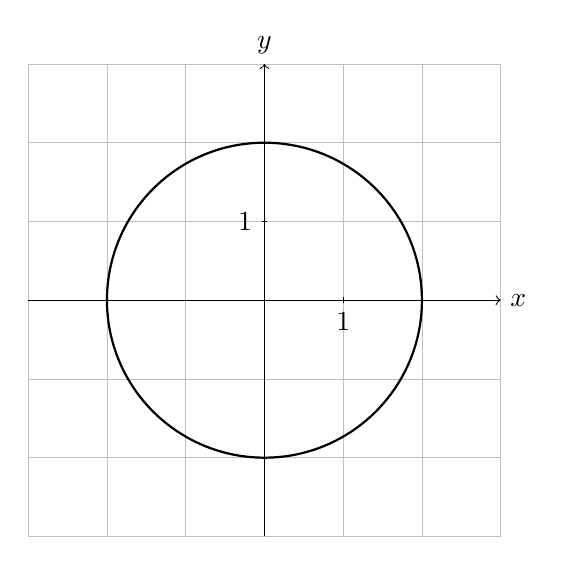
\begin{tikzpicture}
            \draw[step=1cm,gray!50,very thin] (-3,-3) grid (3,3);
            \draw[->] (-3,0)--(3,0) node[right] {$x$};
            \draw[->] (0,-3)--(0,3) node[above] {$y$};
            \foreach \x in {1}
              \draw (\x cm,1pt) -- (\x cm,-1pt) node[anchor=north] {${\x}$};
            \foreach \y in {1}
              \draw (1pt,\y cm) -- (-1pt,\y cm) node[anchor=east] {${\y}$};
            \ifprintanswers
              \draw[thick] (0,0) circle[radius=2];

          \end{tikzpicture}
          \end{center}
          A circle of radius 2 centered at the origin
        \end{solution}
        \item
        {
          Graph the equation $x^{2}+y^{2}=4$ in $\mathbb{R}^{3}$ (i.e. in space).
          Describe it in words.
      
          \textit{Hint:}
          Which values of $z$ satisfy this equation?
        }

          \begin{solution}
            In \(\R^2\) the equation \(x^2+y^2=4\) is a circle of radius 2 in the xy-plane, in other words all points \((x,y)\) that are 2 units away from the origin (the point \((0,0)\)). For instance, the point \((\sqrt{2},\sqrt{2})\).

            In \(\R^3\), for any value of \(z\) the point \((\sqrt{2},\sqrt{2},0)\) also satisfies the equation \(x^2+y^2=4\). Thinking of it like this, you can imagine a circle of radius 2 at every value of \(z\).
            \begin{center}
              \includegraphics[width=.6\textwidth]{12-1-tube.pdf}
            \end{center}
            The cylinder above should extend infinitely in both z-axis directions.
          \end{solution}

        \item
        {
          Graph the equation $z=y^{2}$ in $\mathbb{R}^{3}$.
          Describe it in words.
          \begin{solution}
            \begin{center}
              \includegraphics[width=.6\textwidth]{12-1-z-y3.pdf}
            \end{center}
            The equation represents a parabola in the yz-plane extended infinitely along the x-axis.
          \end{solution}
        }
  \end{enumerate}}
\end{enumerate}
  
\section*{Spheres Leaning Objectives}
  \begin{itemize}
    \item{
      Extend the usual distance equation to three variables.
    }
    \item{
      Draw spheres.
    }
    \item{
      Describe a sphere given its equation
    }
  \end{itemize}
  
\section*{Spheres Examples}
  \begin{definition}
    The distance between points $P_{1}(x_{1},y_{1},z_{1})$ and $P_{2}(x_{2},y_{2},z_{2})$, written $|P_{1}P_{2}|$, is given by
    \[
      |P_{1}P_{2}|=\sqrt{(x_{2}-x_{1})^{2}+(y_{2}-y_{1})^{2}+(z_{2}-z_{1})^{2}}
    \]
  \end{definition}
  
  \begin{enumerate}
    \item{
      Calculate the distance between $(1,2,3)$ and $(3,-1,0)$.
      \begin{solution}
        \begin{align*}
          d\left((1,2,3),(3,-1,0)\right) & = \sqrt{(1-3)^2+(2-(-1))^2+(3-0)^2}\\
            & = \sqrt{4+9+9} = \sqrt{22}
        \end{align*}
      \end{solution}
    }
  \end{enumerate}
  
  \begin{definition}
    The set of all points in $\mathbb{R}^{3}$ equidistant from a center point is called a sphere.
    
    An equation of a sphere with center $C(h,k,l)$ and radius $r$ is
    \[
      (x-h)^{2}+(y-k)^{2}+(z-l)^{2}=r^{2}.
    \]
  \end{definition}
  
  \begin{enumerate}
    \item[2.]{
      Find an equation of the sphere centered at $(1,-2,3)$ with radius $2$.
      \begin{solution}
        Using the above with \(h=1\), \(k=-2\), \(l=3\), and \(r=2\) gives us
        \[
          (x-1)^2+(y+2)^2+(z-3)^2=4
        \]
      \end{solution}
    }
    \item[3.]{
      Describe in words and draw the surface $x^{2}+y^{2}+z^{2}=1$.
      \begin{solution}
        A sphere centered at the origin (the point \((0,0,0)\)) with radius 1.
      \begin{center}
        \includegraphics[width=.6\textwidth]{12-1-sphere.pdf}
      \end{center}
      \end{solution}
    }
    \item[4.]{
      Describe the surface $x^{2}-2x+y^{2}+z^{2}+4z=4$ in words.
    }
    \begin{solution}
      We need to complete the square to rewrite this in the form above.

      \begin{align*}
        x^2-2x\phantom{+(-\frac{2}{2})^2}+y^2+z^2+4z\phantom{+(\frac{4}{2})^2} & = 4\\
      \phantom{x^2-2x}+\left(-\frac{2}{2}\right)^2\phantom{+y^2+z^2+4z}+\left(\frac{4}{2}\right)^2 &\phantom{ = 4} +\left(-\frac{2}{2}\right)^2+\left(\frac{4}{2}\right)^2\\
      x^2-2x+1+y^2+z^2+4z+4 & = 4+1+4\\
      (x-1)^2 + y^2 + (z+2)^2 & = 9
      \end{align*}
      This means the surface is a sphere centered at \((1,0,-2)\) with radius \(3\).
    \end{solution}
  \end{enumerate}
\end{document}